% !TEX root = Stanfill_CoDA.tex
\section{Data Application}\label{sec:data}

We consider electron backscatter diffraction (EBSD) data obtained by scanning a fixed  12.5 $\mu$m $\times$ 10 $\mu$m nickel surface at individual locations spaced 0.2 $\mu$m apart. This scan was repeated 14 times for each location yielding a total of 3,449 observations, \citep{bingham09, bingham10b}. Every observation corresponds to the orientation, expressed as a rotation matrix, of a cubic crystal on the metal surface at a particular location. One goal of processing ESBD data is to identify the main orientation of cubic crystals in the metal, where graphs of cubic crystals with similar orientations constitute ``grains'' on the metal surface, thus making the estimation of the main direction $\bm S$ for a sample of rotations relevant here.

At every location, using the 14 repeat scans  we computed the misorientation angle $|r|=\Rdist(\widehat{\bm{S}}, \bm I_{3\times 3})$ of the four estimators ($\widehat{\bm{S}}= \ProjMean$, $\ProjMedian$, $\GeomMean$, and $\GeomMedian$) to compare resulting differences in the corresponding estimates.  In the following we will focus particularly on the differences between $\ProjMean$ and $\ProjMedian$ as the Riemannian estimators  $\GeomMedian$ and $\GeomMean$ largely agree with their Euclidean counterparts. 

The left hand side of Figure~\ref{fig:grain-map} illustrates the implementation of $\ProjMedian$: each location on the plot is colored according to the mis-orientation angle between  the estimate $\ProjMedian$  and the identity $\bm I_{3\times 3}$ (as an arbitrarily chosen reference point).  The plot shows a distinct spatial structure resembling a grain map. On the right hand side of Figure~\ref{fig:grain-map} we illustrate the difference between $\ProjMean$ and $\ProjMedian$ at each location. The difference in estimates is again defined with respect to the mis-orientation angle between both estimates and locations are colored accordingly. \begin{figure}[h!] %  figure placement: here, top, bottom, or page
   \centering
   \vspace{-.15in}
   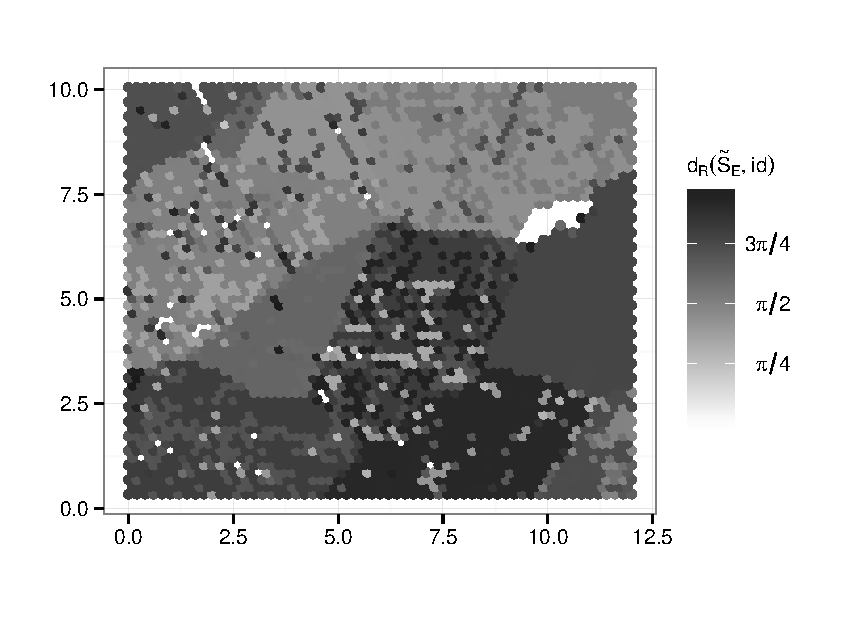
\includegraphics[width=.49\textwidth]{images/grain-map.pdf} 
   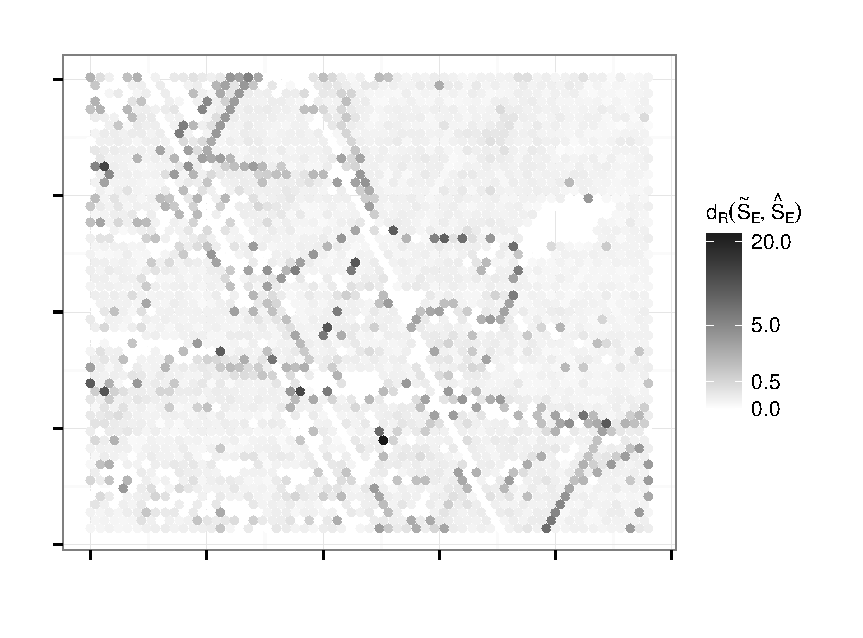
\includegraphics[width=.49\textwidth]{images/grain-diff.pdf} 
    \vspace{-.175in} 
   \caption{ \label{fig:grain-map}  Display of all locations of the investigated nickel surface (left). Each dot corresponds to one location, where shading reflects the angle between $\ProjMedian$ and $\bm I_{3\times 3}$. On the right, differences (in degrees) between $\ProjMedian$ and $\ProjMean$ estimates for each location are shown. Distances of 0.5$^\circ$ or more are generally considered to suggest different main orientations. Note that the mapping of distance to color shading is on a square-root scale.}
\end{figure}
Note that the literature, e.g. \cite{bingham10b}, suggests that distances of $0.5^\circ$ degrees are indicative of different grains. In our example, about 10\% of the locations result in a difference between $\ProjMean$ and $\ProjMedian$ estimates of at least that size. Differences tend to be largest along boundaries between the spatial structures on the left of Figure~\ref{fig:grain-map}  (i.e.~identifying boundaries). 

Table~\ref{tab:rotations} provides an explanation for the observed differences between $\ProjMedian$ and $\ProjMean$ along the spatial structure in Figure~\ref{fig:grain-map}. The table contains the observed orientation (collection of all nine coefficients $x_{ij}$, $1 \le i,j \le 3$, of the $3\times 3$ rotation matrix) for each of the 14 repeated scans at the location with the largest observed difference between $\ProjMedian$ and $\ProjMean$, namely 22.3$^\circ$.   The scans have been re-ordered to better illustrate  the clusters of orientations observed at this particular location. The clusters suggest that, for this location on a ``grain boundary,'' a subset of the scans likely picked up the orientation of a neighboring cubic crystal  belonging to a different grain. A median-type estimator naturally does better for such data with ``outliers'' than a mean-type estimator.  
\begin{table}[h!]
\caption{\label{tab:rotations} List of all rotations in the location with the largest difference between mean and median estimators. We observe one main cluster and one smaller cluster with three additional rotations in the proximity. }
\begin{center}
\scalebox{0.75}{
\begin{tabular}{crrrrrrrrrr}
  \hline
scan& & $x_{11}$ & $x_{12}$& $x_{13}$& $x_{21}$& $x_{22}$& $x_{23}$& $x_{31}$& $x_{32}$& $x_{33}$ \\ 
  \hline
1 & &  -0.646 & -0.552 & -0.527 & 0.464 & -0.833 & 0.303 & -0.606 & -0.049 & 0.794 \\ 
2 & & -0.641 & -0.550 & -0.535 & 0.459 & -0.834 & 0.307 & -0.615 & -0.048 & 0.787 \\ 
3 & & -0.640 & -0.549 & -0.537 & 0.457 & -0.834 & 0.309 & -0.618 & -0.048 & 0.785 \\ 
4 & &  -0.639 & -0.546 & -0.542 & 0.462 & -0.836 & 0.297 & -0.615 & -0.061 & 0.787 \\ 
5 & & -0.639 & -0.547 & -0.540 & 0.456 & -0.835 & 0.307 & -0.619 & -0.050 & 0.783 \\ 
6 & & -0.638 & -0.550 & -0.540 & 0.459 & -0.834 & 0.307 & -0.619 & -0.052 & 0.784 \\ 
7 & & -0.637 & -0.551 & -0.540 & 0.459 & -0.833 & 0.309 & -0.620 & -0.051 & 0.783 \\ 
8 & & -0.633 & -0.554 & -0.540 & 0.464 & -0.830 & 0.309 & -0.619 & -0.055 & 0.783 \\ [5pt]
9 & & -0.068 & -0.422 & -0.904 & 0.994 & -0.105 & 0.025 & -0.084 & -0.900 & 0.427 \\ [5pt]
10 & & -0.017 & -0.633 & -0.774 & 0.961 & -0.224 & 0.162 & -0.276 & -0.741 & 0.612 \\ [5pt]
11 & & -0.005 & -0.551 & -0.834 & 0.982 & -0.158 & 0.099 & -0.186 & -0.819 & 0.542 \\ 
12 & & -0.002 & -0.587 & -0.809 & 0.978 & -0.167 & 0.124 & -0.208 & -0.792 & 0.574 \\ 
13 & & -0.002 & -0.595 & -0.804 & 0.974 & -0.182 & 0.132 & -0.225 & -0.783 & 0.580 \\ [5pt]
14 & & -0.727 & -0.475 & -0.496 & 0.138 & -0.809 & 0.572 & -0.672 & -0.348 & 0.653 \\ 
   \hline
\end{tabular}}
\vspace{-0.5cm}
\end{center}
\end{table}

We visualize Table~\ref{tab:rotations} and the estimates resulting from applying $\ProjMedian$ and $\ProjMean$ at this location in Figure \ref{fig:pcp} using a parallel coordinate plot: for every scan each of the nine coefficients $x_{ij}$ ($1 \le i,j \le 3$)) is plotted separately. Coefficients that correspond to the same scan are connected by a line.   Note that the coefficient values are jittered using a small perturbation in form of a rotation matrix to avoid over-plotting and to illustrate cluster sizes. The light- and dark blue colored line represent the $\ProjMedian$ and $\ProjMean$ estimates of the main direction based on the 14 scans.   This example  illustrates that the median estimate, $\ProjMedian$,  can more reliably estimate the main direction in the presence of potential anomalies on the spatial boundaries of grains.


%\begin{figure}[htbp] %  figure placement: here, top, bottom, or page
%   \centering
%   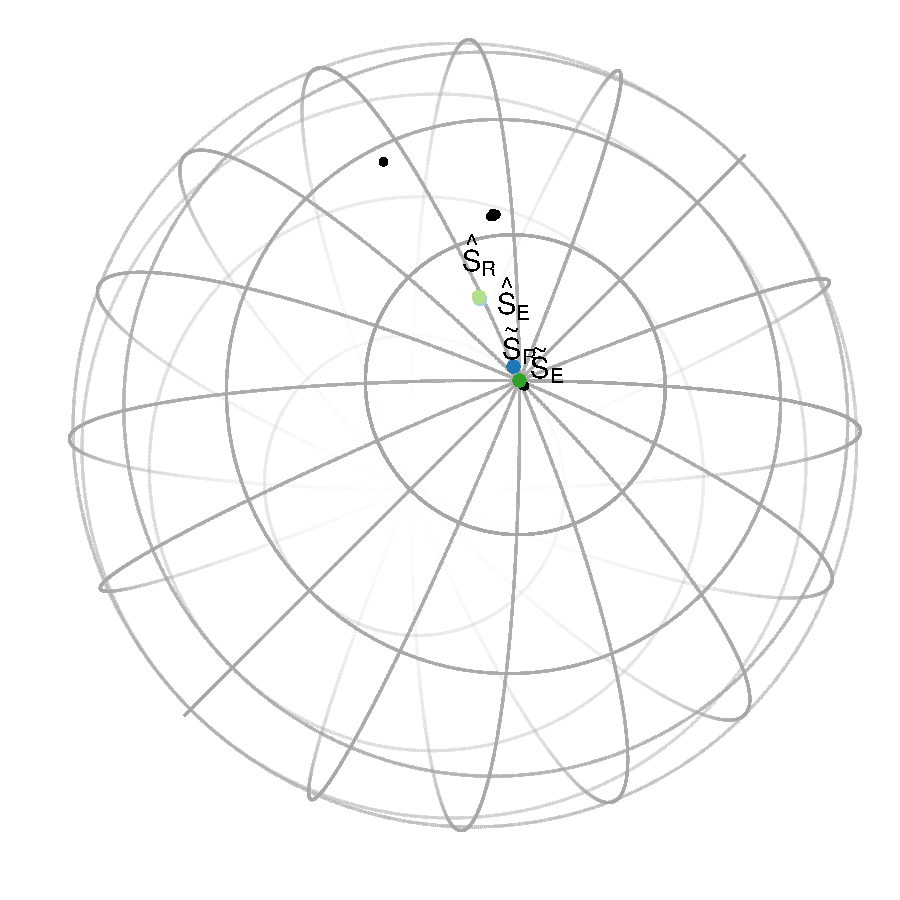
\includegraphics[width=.275\textwidth]{images/eyeball-1031-1.pdf} 
%   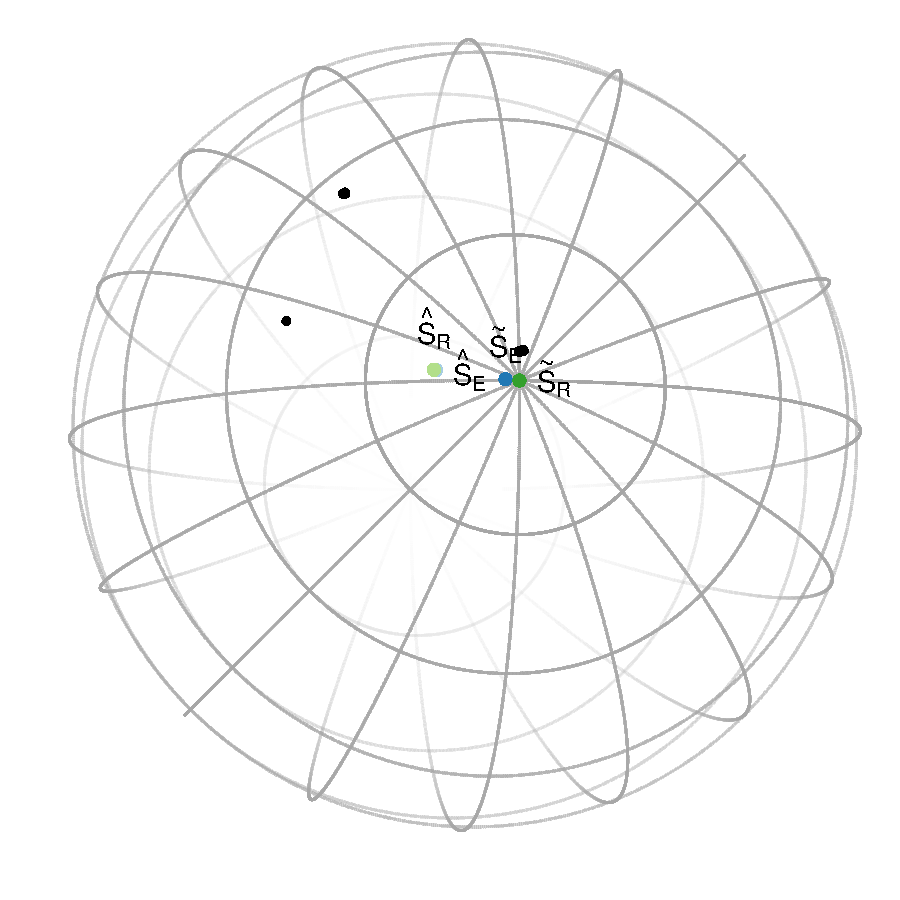
\includegraphics[width=.275\textwidth]{images/eyeball-1031-2.pdf} 
%   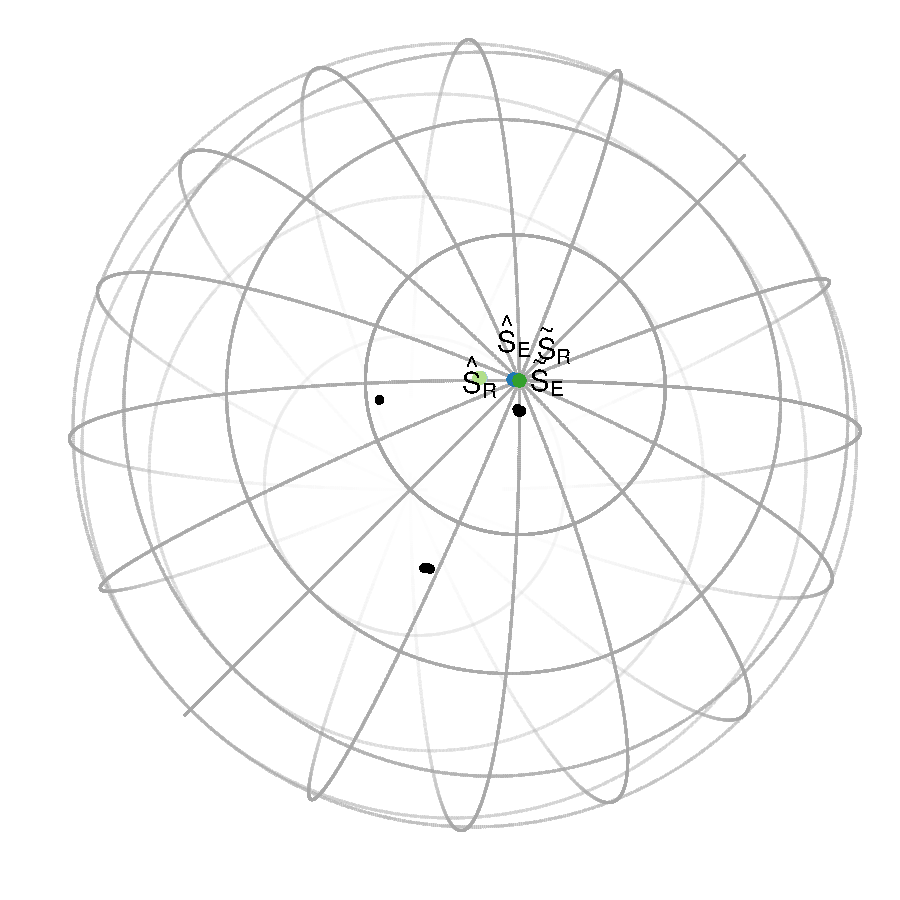
\includegraphics[width=.275\textwidth]{images/eyeball-1031-3.pdf} 
%   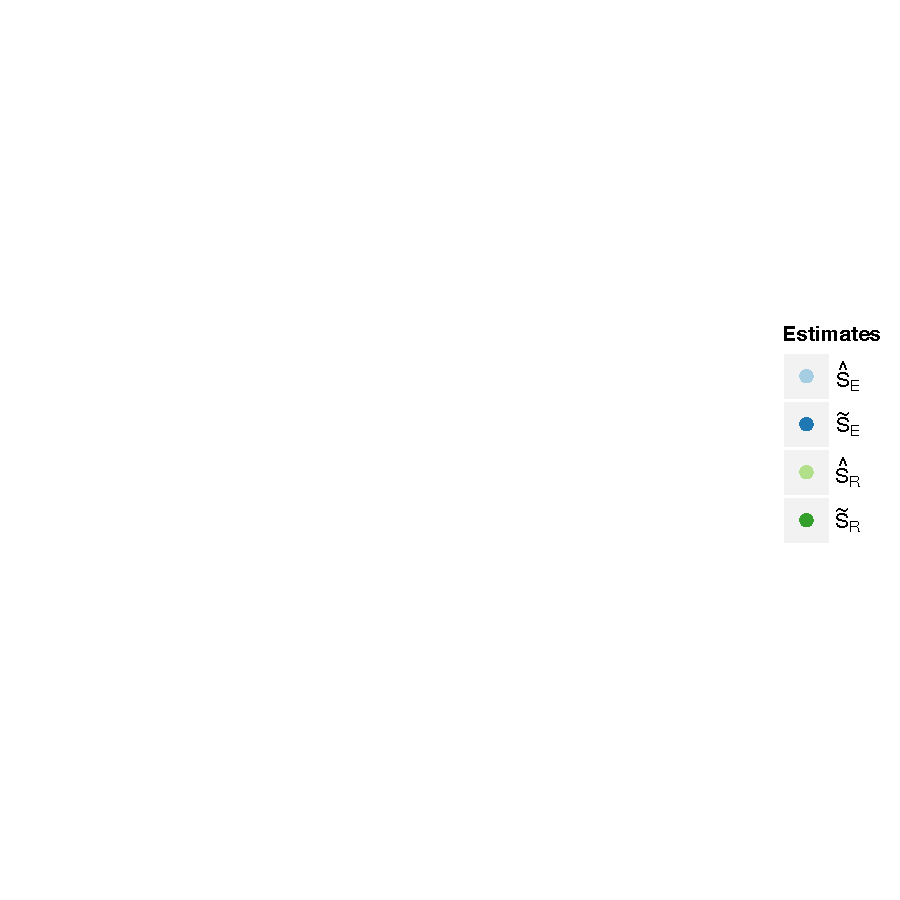
\includegraphics[height=.275\textwidth]{images/legend.pdf} 
%   \caption{ \label{fig:eyeballs-1}Sphere plots of EBSD measurements at a single location. The data sample is shown as dark grey points, the estimates of the main direction are colored and labelled. The clustering of the results makes the existence  of several main directions  quite obvious. }
%\end{figure}

\begin{figure}[htbp] %  figure placement: here, top, bottom, or page
   \centering
   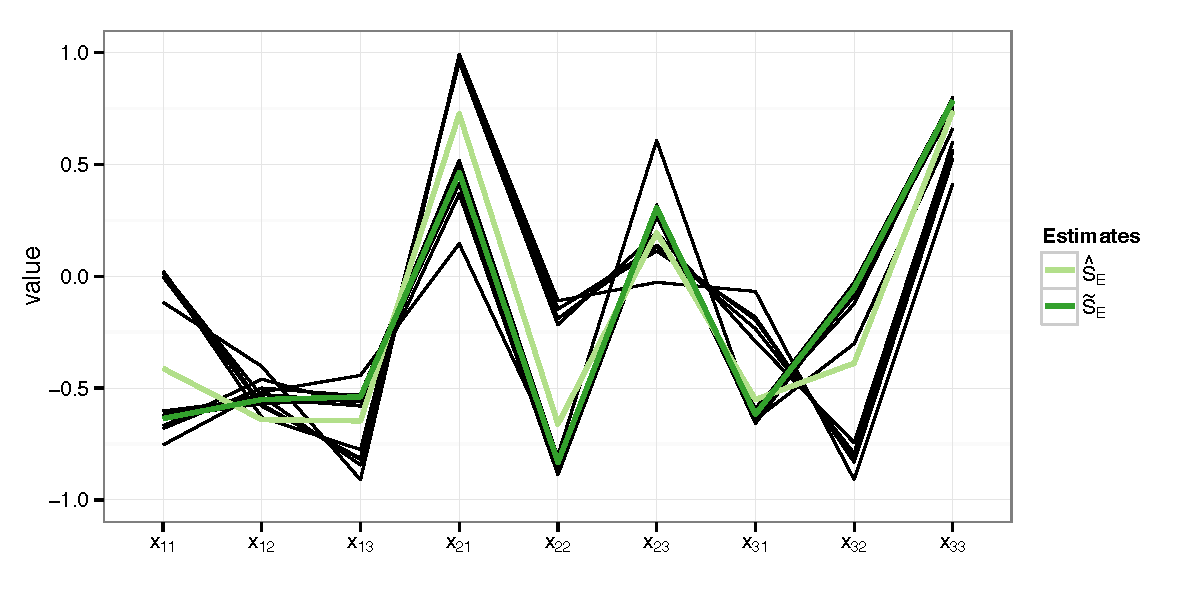
\includegraphics[width=.7\textwidth]{images/pcp.pdf} 
   \caption{ \label{fig:pcp}Parallel coordinate plot of all nine coefficients of the rotation matrices in a single location. }
\end{figure}

%=======
%% !TEX root = Stanfill_CoDA.tex
%\section{Data Application}\label{sec:data}
%
%We consider electron backscatter diffraction (EBSD) data obtained by scanning a fixed  12.5 $\mu$m $\times$ 10 $\mu$m nickel surface at individual locations spaced 0.2 $\mu$m apart. This scan was repeated 14 times for each location yielding a total of 3,449 observations, \citep{bingham09, bingham10b}. Every observation corresponds to the orientation, expressed as a rotation matrix, of a cubic crystal in the metal at a particular location. One goal of analyzing ESBD data is to identify the main orientation of cubic crystals in the metal, thus making the estimation of the main direction $\bm S$ for a sample of rotations important to the field.\\
%
%At every location we implemented each of the four estimators ($\ProjMean$, $\ProjMedian$, $\GeomMean$, and $\GeomMedian$) to compare resulting differences in the corresponding estimates.  In the following we will focus particularly on the differences between $\ProjMean$ and $\ProjMedian$ as the Riemannian estimators  $\GeomMedian$ and $\GeomMean$ largely agree with their Euclidean counterparts. 
%
%The left hand side of Figure~\ref{fig:grain-map} illustrates the implementation of $\ProjMedian$: each location on the plot is colored according to the mis-orientation angle between $\ProjMedian$  and the identity $\bm I_{3\times 3}$ (as an arbitrarily chosen reference point).  The plot shows a distinct spatial structure \blue{resembling a grain map}. On the right hand side of Figure~\ref{fig:grain-map} we illustrate the difference between $\ProjMean$ and $\ProjMedian$ at each location. The difference in estimates is again defined with respect to the mis-orientation angle between both estimates and locations are colored accordingly. Note that the literature, e.g. \cite{bingham10b}, suggests that distances of $0.5^\circ$ degrees are indicative of different grains. In our example, about 10\% of the locations result in a difference between $\ProjMean$ and $\ProjMedian$ estimates of at least that size. Differences tend to be largest along boundaries between the spatial structures on the left of Figure~\ref{fig:grain-map}.  
%\begin{figure}[htbp] %  figure placement: here, top, bottom, or page
%   \centering
%   \vspace{-.15in}
%   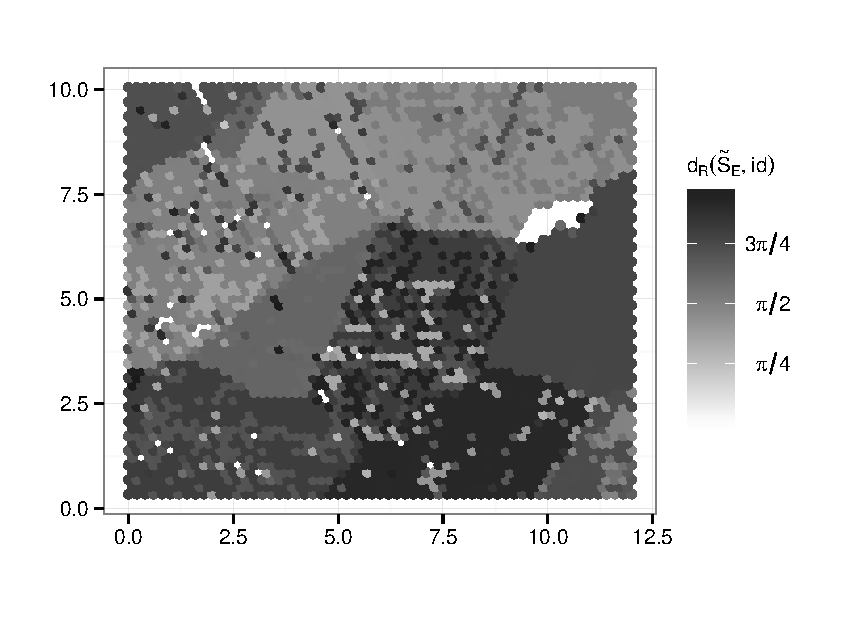
\includegraphics[width=.49\textwidth]{images/grain-map.pdf} 
%   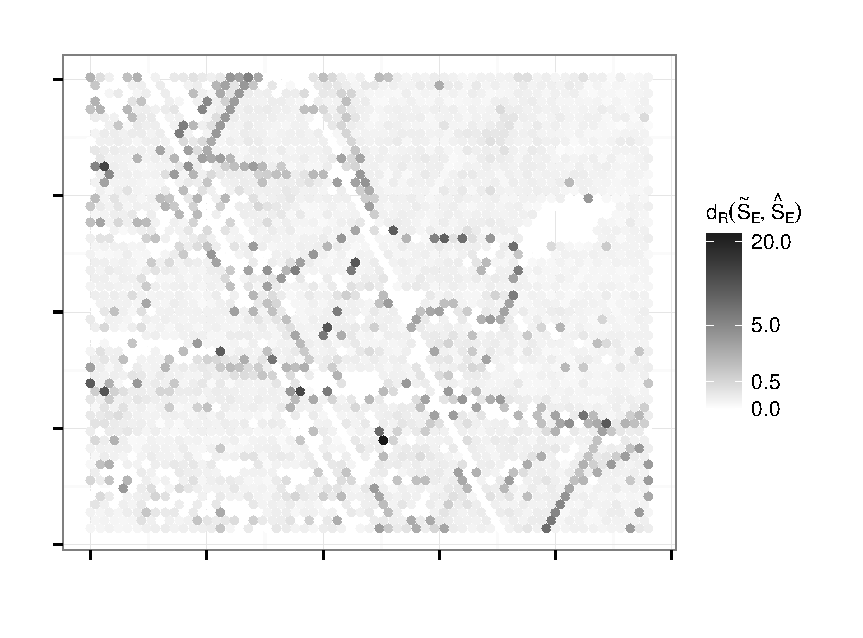
\includegraphics[width=.49\textwidth]{images/grain-diff.pdf} 
%    \vspace{-.175in} 
%   \caption{ \label{fig:grain-map}  Display of all locations of the investigated nickel surface (left). Each dot corresponds to one location, where shading reflects the angle between $\ProjMedian$ and $\bm I_{3\times 3}$. On the right, differences (in degrees) between $\ProjMedian$ and $\ProjMean$ estimates for each location are shown. Distances of 0.5$^\circ$ or more are generally considered to suggest different main orientations. Note that the mapping of distance to color shading is on a square-root scale.}
%\end{figure}
%Table~\ref{tab:rotations} provides an explanation for the observed differences between $\ProjMedian$ and $\ProjMean$ along the spatial structure in Figure~\ref{fig:grain-map}. The table contains the observed orientation (collection of all nine coefficients $x_{ij}$, $1 \le i,j \le 3$, of the $3\times 3$ rotation matrix) for each of the 14 repeated scans at the location with the largest observed difference between $\ProjMedian$ and $\ProjMean$, namely 22.3$^\circ$.   The scans have been re-ordered to better illustrate  three clusters of orientations observed at this particular location. The clusters suggest that for a subset of the scans the orientation from a neighboring cubic crystal, likely belonging to a different grain, was picked up instead of the orientation of the   target cubic crystal. A median-type estimator naturally does better for such data than a mean-type estimator.  
%\begin{table}[h!]
%\caption{\label{tab:rotations} List of all rotations in the location with the largest difference between mean and median estimators. We observe one main cluster and one smaller cluster with three additional rotations in the proximity. }
%\begin{center}
%\scalebox{0.75}{
%\begin{tabular}{crrrrrrrrrr}
%  \hline
%scan& & $x_{11}$ & $x_{12}$& $x_{13}$& $x_{21}$& $x_{22}$& $x_{23}$& $x_{31}$& $x_{32}$& $x_{33}$ \\ 
%  \hline
%1 & &  -0.646 & -0.552 & -0.527 & 0.464 & -0.833 & 0.303 & -0.606 & -0.049 & 0.794 \\ 
%2 & & -0.641 & -0.550 & -0.535 & 0.459 & -0.834 & 0.307 & -0.615 & -0.048 & 0.787 \\ 
%3 & & -0.640 & -0.549 & -0.537 & 0.457 & -0.834 & 0.309 & -0.618 & -0.048 & 0.785 \\ 
%4 & &  -0.639 & -0.546 & -0.542 & 0.462 & -0.836 & 0.297 & -0.615 & -0.061 & 0.787 \\ 
%5 & & -0.639 & -0.547 & -0.540 & 0.456 & -0.835 & 0.307 & -0.619 & -0.050 & 0.783 \\ 
%6 & & -0.638 & -0.550 & -0.540 & 0.459 & -0.834 & 0.307 & -0.619 & -0.052 & 0.784 \\ 
%7 & & -0.637 & -0.551 & -0.540 & 0.459 & -0.833 & 0.309 & -0.620 & -0.051 & 0.783 \\ 
%8 & & -0.633 & -0.554 & -0.540 & 0.464 & -0.830 & 0.309 & -0.619 & -0.055 & 0.783 \\ [5pt]
%9 & & -0.068 & -0.422 & -0.904 & 0.994 & -0.105 & 0.025 & -0.084 & -0.900 & 0.427 \\ [5pt]
%10 & & -0.017 & -0.633 & -0.774 & 0.961 & -0.224 & 0.162 & -0.276 & -0.741 & 0.612 \\ [5pt]
%11 & & -0.005 & -0.551 & -0.834 & 0.982 & -0.158 & 0.099 & -0.186 & -0.819 & 0.542 \\ 
%12 & & -0.002 & -0.587 & -0.809 & 0.978 & -0.167 & 0.124 & -0.208 & -0.792 & 0.574 \\ 
%13 & & -0.002 & -0.595 & -0.804 & 0.974 & -0.182 & 0.132 & -0.225 & -0.783 & 0.580 \\ [5pt]
%14 & & -0.727 & -0.475 & -0.496 & 0.138 & -0.809 & 0.572 & -0.672 & -0.348 & 0.653 \\ 
%   \hline
%\end{tabular}}
%\vspace{-0.5cm}
%\end{center}
%\end{table}
%
%  
%We visualize Table~\ref{tab:rotations} and the estimates resulting from applying $\ProjMedian$ and $\ProjMean$ at this location in Figure \ref{fig:pcp} using a parallel coordinate plot: for every scan each of the nine coefficients $x_{ij}$ ($1 \le i,j \le 3$)) is plotted separately. Coefficients that correspond to the same scan are connected by a line.   Note that the coefficient values are jittered using a small perturbation in form of a rotation matrix to avoid over-plotting and to illustrate cluster sizes. The light- and dark blue colored line represent the $\ProjMedian$ and $\ProjMean$ estimates of the main direction based on the 14 scans.   
%%Note that the figure shows a sample of a single location, yet the clustering in the data suggests clearly the presence of \emph{several} main directions. The same holds true for locations in the vicinity which happen to coincide with grain boundaries. 
%
%This example  illustrates that the median estimate, $\ProjMedian$,  can more reliably estimate the main direction in the presence of \red{clustered data}.
%
%
%%\begin{figure}[htbp] %  figure placement: here, top, bottom, or page
%%   \centering
%%   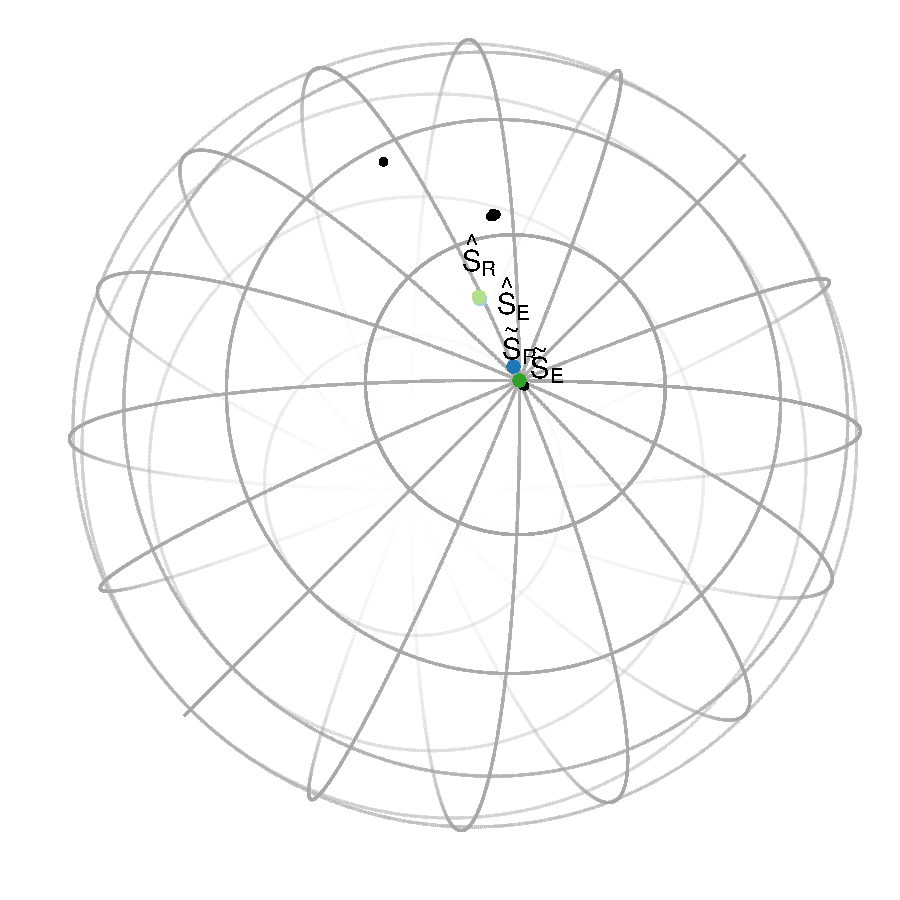
\includegraphics[width=.275\textwidth]{images/eyeball-1031-1.pdf} 
%%   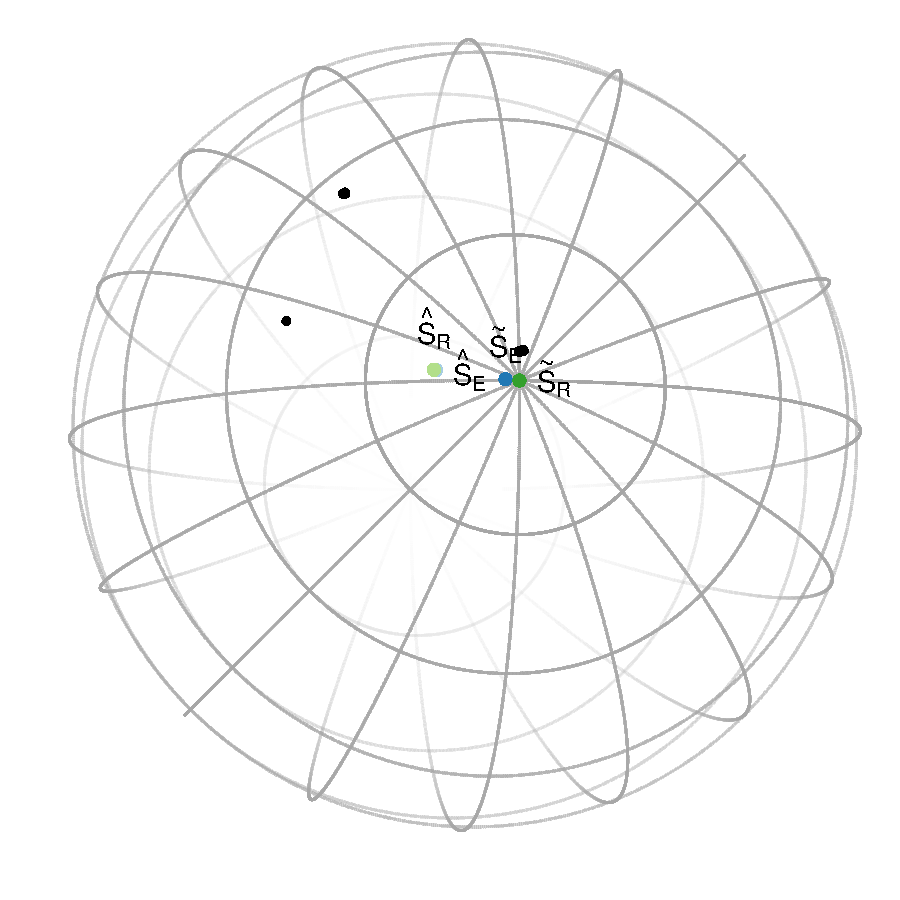
\includegraphics[width=.275\textwidth]{images/eyeball-1031-2.pdf} 
%%   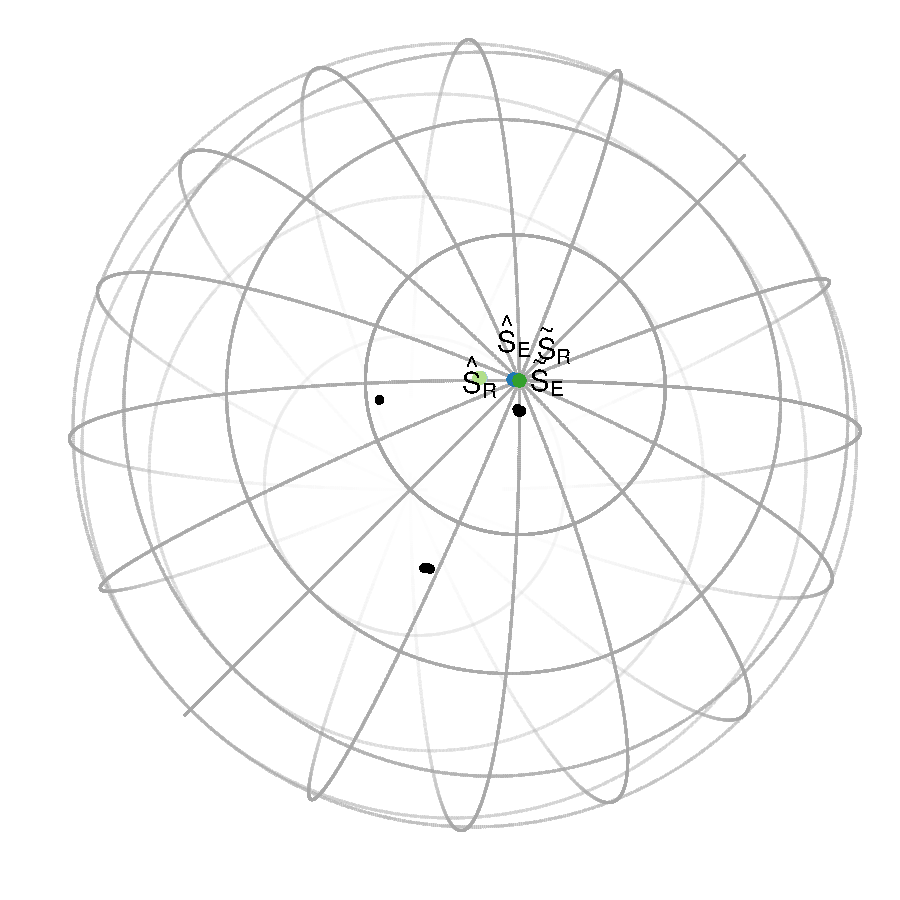
\includegraphics[width=.275\textwidth]{images/eyeball-1031-3.pdf} 
%%   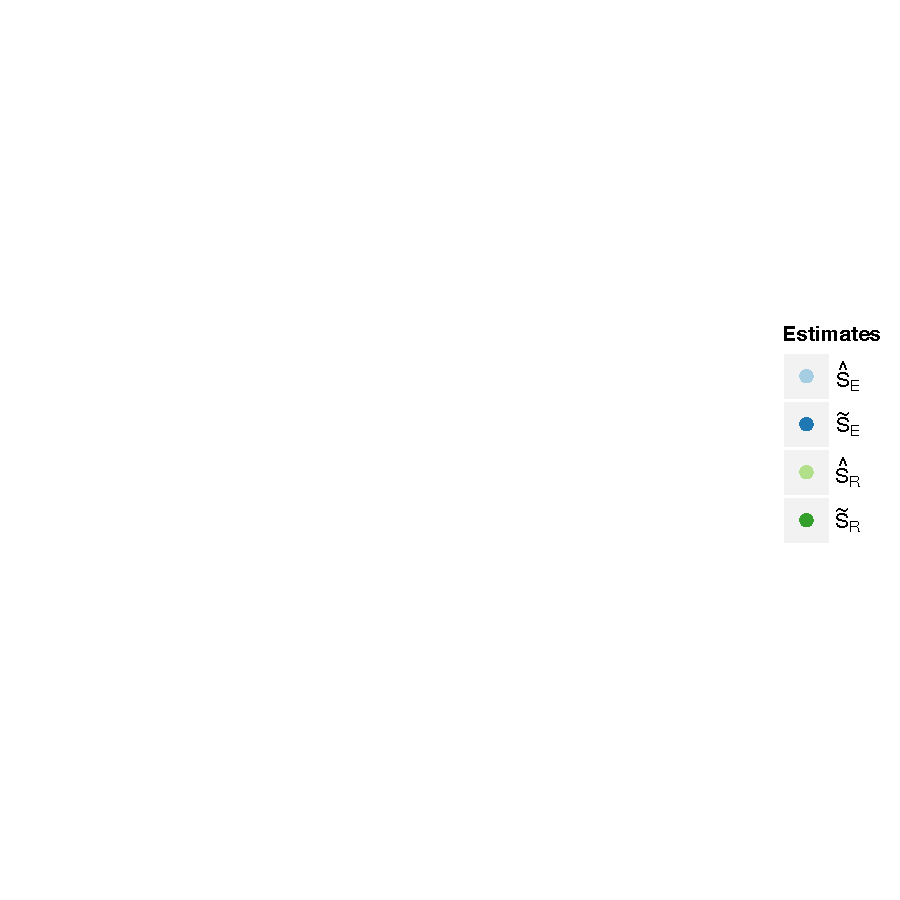
\includegraphics[height=.275\textwidth]{images/legend.pdf} 
%%   \caption{ \label{fig:eyeballs-1}Sphere plots of EBSD measurements at a single location. The data sample is shown as dark grey points, the estimates of the main direction are colored and labelled. The clustering of the results makes the existence  of several main directions  quite obvious. }
%%\end{figure}
%
%\begin{figure}[htbp] %  figure placement: here, top, bottom, or page
%   \centering
%   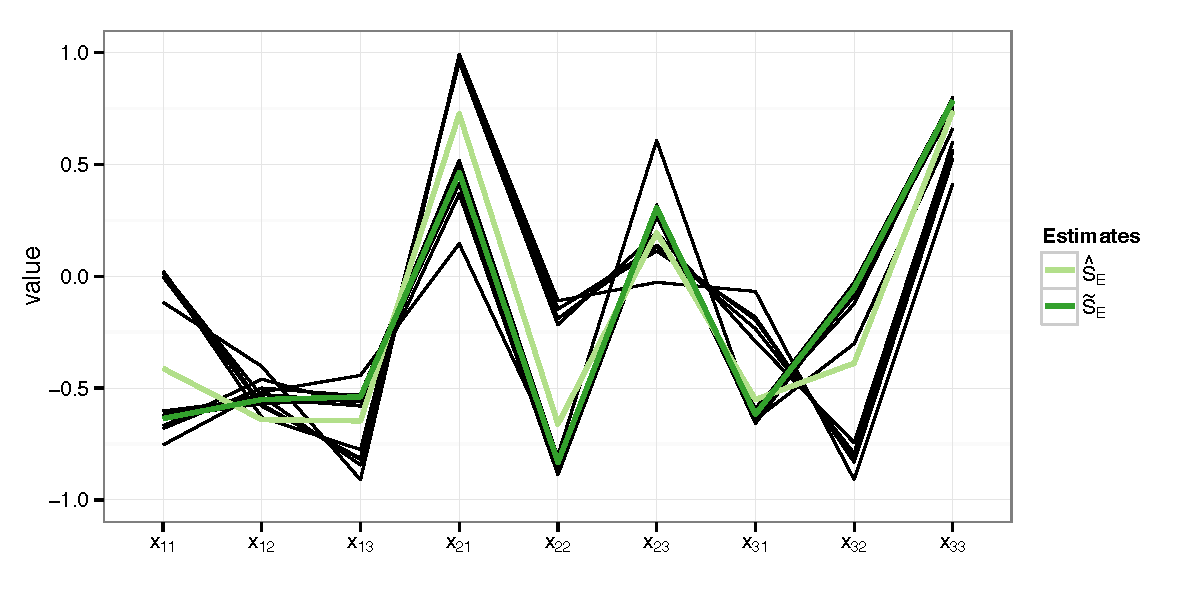
\includegraphics[width=.7\textwidth]{images/pcp.pdf} 
%   \caption{ \label{fig:pcp}Parallel coordinate plot of all nine coefficients of the rotation matrices in a single location. }
%\end{figure}
%
%>>>>>>> 2ae524a3512a18ca58f9808d9a1c66a11687f0c3
